\documentclass[unicode,11pt,a4paper,oneside,numbers=endperiod,openany]{scrartcl}

\usepackage{ifthen}
\usepackage[utf8]{inputenc}
\usepackage{graphics}
\usepackage{graphicx}
\usepackage{float}
\usepackage{hyperref}

\pagestyle{plain}
\voffset -5mm
\oddsidemargin  -2.5mm
\evensidemargin 0mm
\marginparwidth 2cm
\marginparsep 0pt
\topmargin 0mm
\headheight 0pt
\headsep 0pt
\topskip 0pt        
\textheight 255mm
\textwidth 165mm

\newcommand{\duedate} {}
\newcommand{\setduedate}[1]{%
\renewcommand\duedate {#1}}
\newcommand\isassignment {false}
\newcommand{\setassignment}{\renewcommand\isassignment {true}}
\newcommand{\ifassignment}[1]{\ifthenelse{\boolean{\isassignment}}{#1}{}}
\newcommand{\ifnotassignment}[1]{\ifthenelse{\boolean{\isassignment}}{}{#1}}

\newcommand\serieheader[6]{
\thispagestyle{empty}%
\begin{flushleft}

\includegraphics[width=\textwidth]{./assets/logo-info.pdf}
\end{flushleft}
  {\large\ignorespaces #3 \hspace{\fill}\ignorespaces #4}\\
  \noindent%
  \bigskip
  \hrule\par\bigskip\noindent%
  \bigskip {\ignorespaces {\Large{\textbf{#5}}}
  \hspace{\fill}\ignorespaces \large \ifthenelse{\boolean{\isassignment}}{\duedate}{#6}}
  \hrule\par\bigskip\noindent%  \linebreak
 }

\makeatletter
\def\enumerateMod{\ifnum \@enumdepth >3 \@toodeep\else
      \advance\@enumdepth \@ne
      \edef\@enumctr{enum\romannumeral\the\@enumdepth}\list
      {\csname label\@enumctr\endcsname}{\usecounter
        {\@enumctr}%%%? the following differs from "enumerate"
	\topsep0pt%
	\partopsep0pt%
	\itemsep0pt%
	\def\makelabel##1{\hss\llap{##1}}}\fi}
\let\endenumerateMod =\endlist
\makeatother

\usepackage{textcomp}


\begin{document}

\graphicspath{ {./assets/} }

\setassignment
\setduedate{Final Report}

\serieheader{Numerical Computing}{2021}{Student: Edoardo Riggio}{}{Hotel Search}{}
\newline

\tableofcontents

\newpage

\section{Abstract}
In this project I have to create a search engine for hotels. These hotels must be taken from at least two different countries and from several different websites -- i.e. more than a couple. After having scraped the hotels using Scrapy, I have to index them using Solr and display them to the user via a graphical user interface. Moreover, the top 20 results must be visualized onto a map. \\ \\
The project is structured in four main parts: Crawling, Indexing, Visualizing and User Evaluation. For each of the parts -- except User Evaluation -- I have created a repository on \underline{\href{https://github.com/hotel-se}{GitHub}}.

\section{Crawling}
The fist part of the project consisted in crawling several websites in order to get data on hotels. In order to do so I've only used Scrapy. I've crawled hotels in Switzerland and Italy from three different websites. These websites are:

\begin{enumerate}
	\item Tripadvisor
	\item Lonely Planet
	\item MySwitzerland
\end{enumerate}
The crawled data was then structured as follows:

\begin{table}[H]
	\centering
	\begin{tabular}{|l|l|l|} \hline 
		\textbf{Element} & \textbf{Type} & \textbf{Description}  \\ \hline
		Source & String & Where is the hotel from -- tripadvisor $|$ lonely $|$ myswitzerland \\
		Name & String & The name of the hotel \\
		URL & String & The url of the hotel detail page \\
		Address & String & The physical address of the hotel \\
		Coordinates & String & The coordinates of the hotel in the format \textit{lat,lon} \\
		Phone\_Number & String & The phone number of the hotel \\
		Description & String & The description of the hotel \\
		Rating.Score & String & The rating of the hotel out of 4 \\
		Rating.N\_Ratings & String & The number of people who rated the hotel \\
		\hline
	\end{tabular}
\end{table}

\noindent The coordinates where the only element that was not taken from the websites -- being maps rendered dynamically. I have used a free and open-source API called \textit{nominatim} in order to convert all of the addresses into coordinates. The only problem with this method is that not all addresses are interpreted correctly by the API, thus some hotels will have \textit{null} values for the coordinates. \\ \\
The reason I didn't choose Booking.com -- as it was suggested in the project pdf -- was because I had a weird bug with the spider where it generated multiple copies of already scraped hotels. For this reason I decided to use MySwitzerland instead. \\ \\
All of the data obtained from the spiders has been saved in three different JSON files -- one for each spider -- inside of the crawler repository. From these three websites I've obtained 10'020 hotels. Of them, 6'529 hotel are in Switzerland, and 3'491 are in Italy.

\subsection{Tripadvisor}
In order to scrape hotels from Tripadvisor, I started to scrape from

\begin{verbatim}
  https://www.tripadvisor.com/Hotels-g187768-Italy-Hotels.html
\end{verbatim}
And

\begin{verbatim}
  https://www.tripadvisor.com/Hotels-g188045-Switzerland-Hotels.html
\end{verbatim}
Rather than from \verb|https://www.tripadvisor.com|. This is because those two links directly have a list of the hotels in the respective country, thus there is no need for further requests in order to navigate to those pages. \\ \\
This website was simple to scrape, and the data was displayed in a structured way. The only problem I had with this website was how to move to the next page. To do so I had to send a \verb|POST| request to Tripadvisor servers which had to contain a user-agent -- without which I couldn't get the actual next page, and a parameter called \verb|offset|. This parameter needed to be set to a multiple of 25 -- 25 for page 2, 50 for page 3...

\subsection{Lonely Planet}
In order to scrape this website -- like in the case of Tripadvisor -- I had to start from

\begin{verbatim}
  https://www.lonelyplanet.com/italy/hotels?page=1&subtypes=Hotel
\end{verbatim}
And

\begin{verbatim}
  https://www.lonelyplanet.com/switzerland/hotels?page=1&subtypes=Hotel
\end{verbatim}
Rather than  from \verb|https://www.lonelyplanet.com|. This website was easy to scrape and well structured, thus no problems were encountered.

\subsection{MySwitzerland}
In order to scrape this website I started from

\begin{verbatim}
  https://www.myswitzerland.com/en-ch/accommodations/hotel-search/
\end{verbatim}
Rather than \verb|https://www.myswitzerland.com|. As for the scraping of this website, I didn't encounter any problem, thus no particular workaround or hack was needed.

\section{Indexing}
In order to index the data, I've used Solr. In Solr the first thing I did was to modify the default \textit{managed-schema} contained inside of the \textit{config} folder of the \textit{$\_$default} schema. This was done in order to let Solr know how to interpret the data passed to it. The data is divided in Solr in the following fields:

\begin{table}[H]
	\centering
	\begin{tabular}{|l|l|} \hline 
		\textbf{Element} & \textbf{Type}  \\ \hline
		Source & string \\
		Name & string \\
		URL & string \\
		Address & string \\
		Coordinates & location \\
		Phone\_Number & string \\
		Description & string \\
		Rating.Score & pdouble \\
		Rating.N\_Ratings & string \\
		$\_$text$\_$ & text$\_$general \\
		\hline
	\end{tabular}
\end{table}
\noindent The coordinates of each hotel are saved as a \textit{location}. By doing so, I am able to make requests to Solr based on the distance between the place the user has searched for and the hotels. \\ \\
Moreover, as I've said when talking about crawling, not all locations will have coordinates -- since I'm relying on an external API. For this reason I've decided to add a field called \textit{$\_$text$\_$}, which matches text from both the \textit{url} field, as well as the \textit{address} field. In this way, in the case that a hotel does not have coordinates, it will be matched based on whether the query is found inside either the \textit{url} or \textit{address} fields. \\ \\
The reason why I've chosen to match the query to the \textit{url} field, is that the urls taken from all three sources -- Tripadvisor, Lonely Planet and MySwitzerland -- most of the time contain the place where the hotel is located in.

\subsection{Query}
In order to retrieve the most relevant data from the Solr database, I've used the following query -- which uses Solr spacial search:

\begin{verbatim}
 d=5&fq=%7B!geofilt%7D&pt={lat}%2C{lon}&q={query}&rows=25&sfield=coordinates
  &sort=geodist()%20asc
\end{verbatim}
Breaking down this long query, we can see the following parameters being passed to Solr:

\begin{itemize}
	\item \textbf{fq=\%7B!geofilt\%7D} $\rightarrow$ \textbf{fq=\{!geofilt\}}
	\vspace{.2cm} \\
	This sets the filtering method of the query to be the Solr geofiltering function -- which takes \textit{sfield}, \textit{d} and \textit{pt} as parameters.
	
	\item \textbf{d=5}
	\vspace{.2cm} \\
	This sets the distance of the hotel coordinates to be in a 5km radius from the center -- which is defined later in the query.
	
	\item \textbf{pt=\{lat\}\%2C\{lon\}} $\rightarrow$ \textbf{pt=\{lat\},\{lon\}}
	\vspace{.2cm} \\
	This sets the center point for the filtering to be the one defined by the coordinates \textit{lat} and \textit{lon}.
	
	\item \textbf{sfield=coordinates}
	\vspace{.2cm} \\
	This tells Solr that the field of type \textit{location} is the \textit{coordinates} field.
	
	\item \textbf{q=\{query\}}
	\vspace{.2cm} \\
	This sets the query to be the name of the place being searched for. This becomes very useful in the case that the coordinates of a hotel are not present.
	
	\item \textbf{sort=geodist()\%20asc} $\rightarrow$ \textbf{sort=geodist() asc}
	\vspace{.2cm} \\
	This sets the sorting function to be \textit{geodist()} -- which will sort all of the data based on their distance to \textit{pt}. The value \textit{asc} indicates that the sorted data needs to be in ascending order of distance.
\end{itemize}

\subsection{CORS Policy}
Solr serves as a backend for the website, thus needs to be always active in order to receive queries and send out responses. The only problem I've encountered with this server was that the CORS (Cross-Origin Resource Sharing) header is by default not active. \\ \\
In order to fix this problem, I've modified the file:

\begin{verbatim}
  solr-8.10.1/server/solr-webapp/webapp/WEB-INF/web.xml
\end{verbatim}
By adding a \textit{filter} tag and a \textit{filter-mapping}. By doing so, I'm activating the CORS header making it possible for the frontend to connect to the Solr server.

\section{Webapp}
In order to create the webapp, I've used Vue.js. Vue is a JavaScript framework used to create modular applications, and is particularly suitable when dealing with lists -- in this case the hotels. \\ \\
The website is divided in three main pages. The first is used to search for a place, the second is used to both display the results and let the user modify the query, and the third is used to warn the user that his/her query didn't produce any result.

\subsection{Search Page}
This page was left very bare-bones intentionally. This is because I wanted to make the user focus only on what he/she came on the website to do: search for hotels. \\ \\
After that the user has typed in the search box the location to look for and pressed enter, the website will make a fetch request to \textit{nominatim} -- in order to get the coordinates of the location to look for -- and to Solr -- in order to fetch all of the hotels that are geographically closer to the searched location. \\ \\
The following is a screen-shot of the page.

\begin{center}
	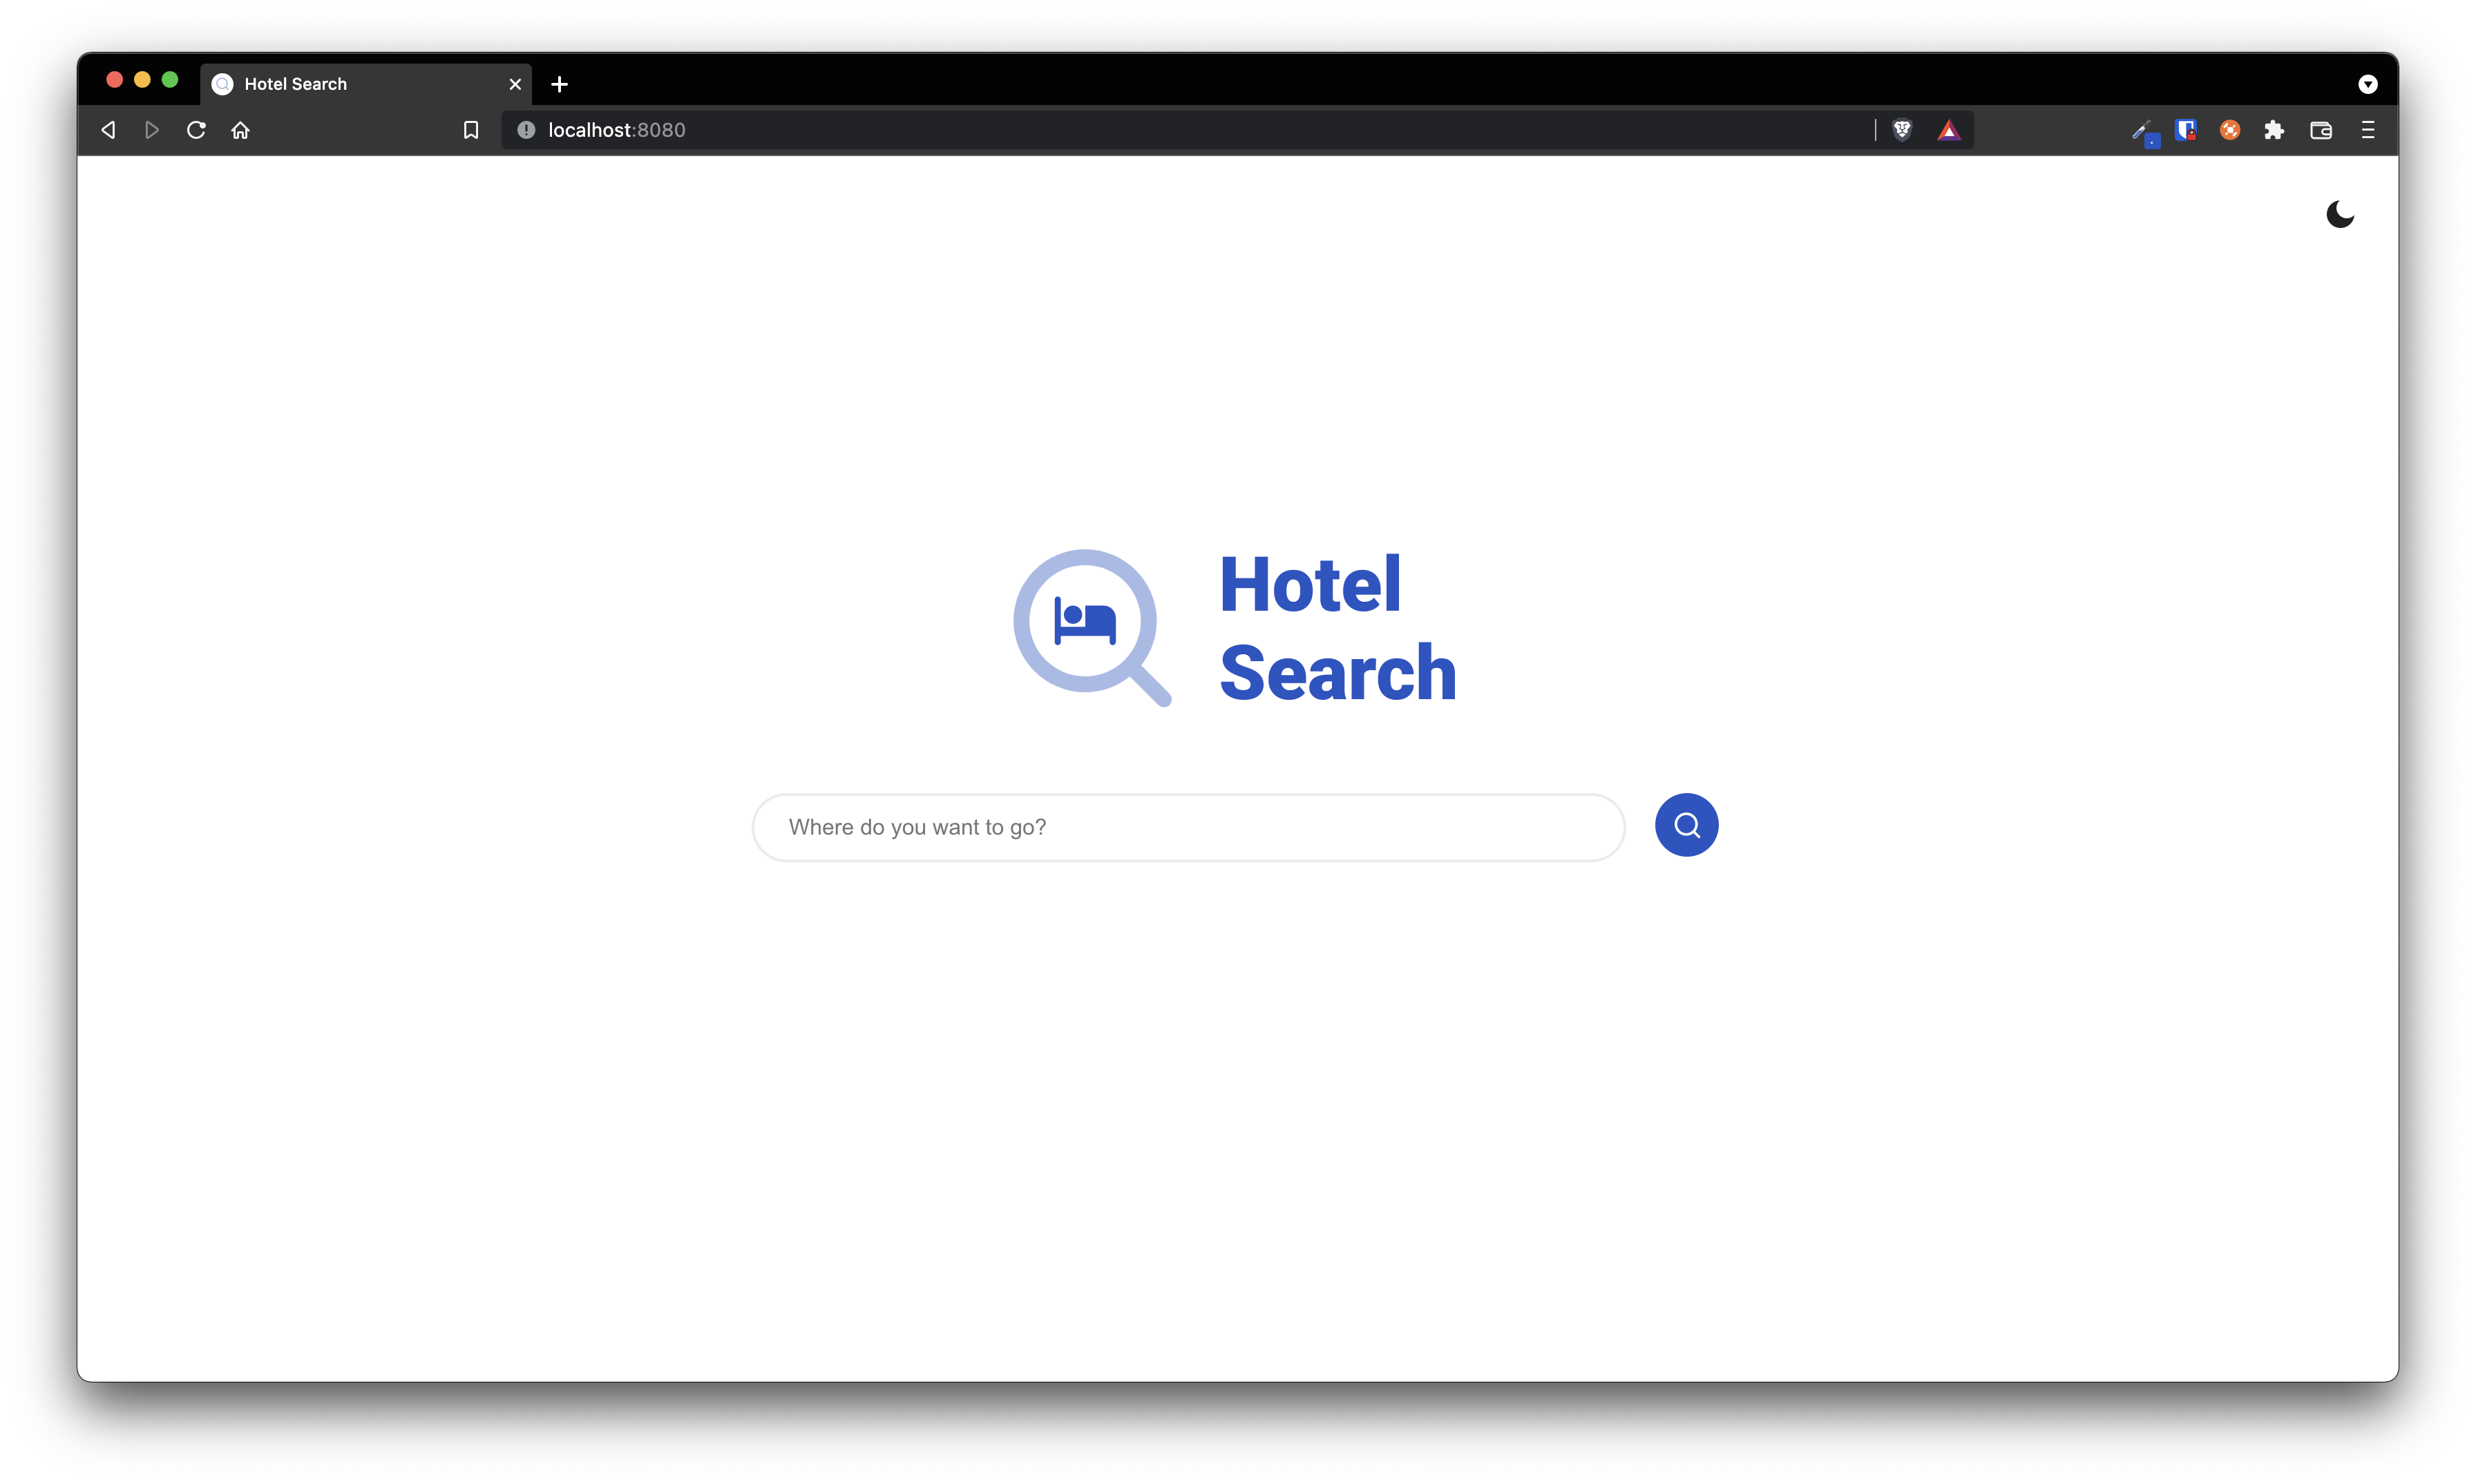
\includegraphics[width=12cm]{./main.png}
\end{center}

\subsection{Results Page}
In this page all of the results are displayed. In addition to that -- as per requirements -- I've included also a map that displays the top twenty results of the query. Finally, this page can be also used in order to refine the query or completely change it. \\ \\
In order to display the map and the markers, I've used an \textit{openstreetmaps} wrapper for Vue. The map is interactive, and if hovered, the markers will show some information -- name and address -- of the respective hotel. The reason behind showing only the name and the address in the tool-tip of the marker, is that more information would have resulted in a bigger tool-tip and a less aesthetically pleasing design. Moreover, all of the information relative to every single hotel is displayed under the map. \\ \\
Every hotel has the following data:

\begin{itemize}
	\item \textbf{Address}
	\item \textbf{Name}
	\item \textbf{Two-Line Description}
	\item \textbf{Rating}
	\item \textbf{Source}
\end{itemize}
The number of hotels retrieved from Solr, and how much time the request took, can be found right under the map. Moreover, only 25 results are displayed per page. For this reason, I've also implemented a pagination system. \\ \\
The following is a screen-shot of the page.

\begin{center}
	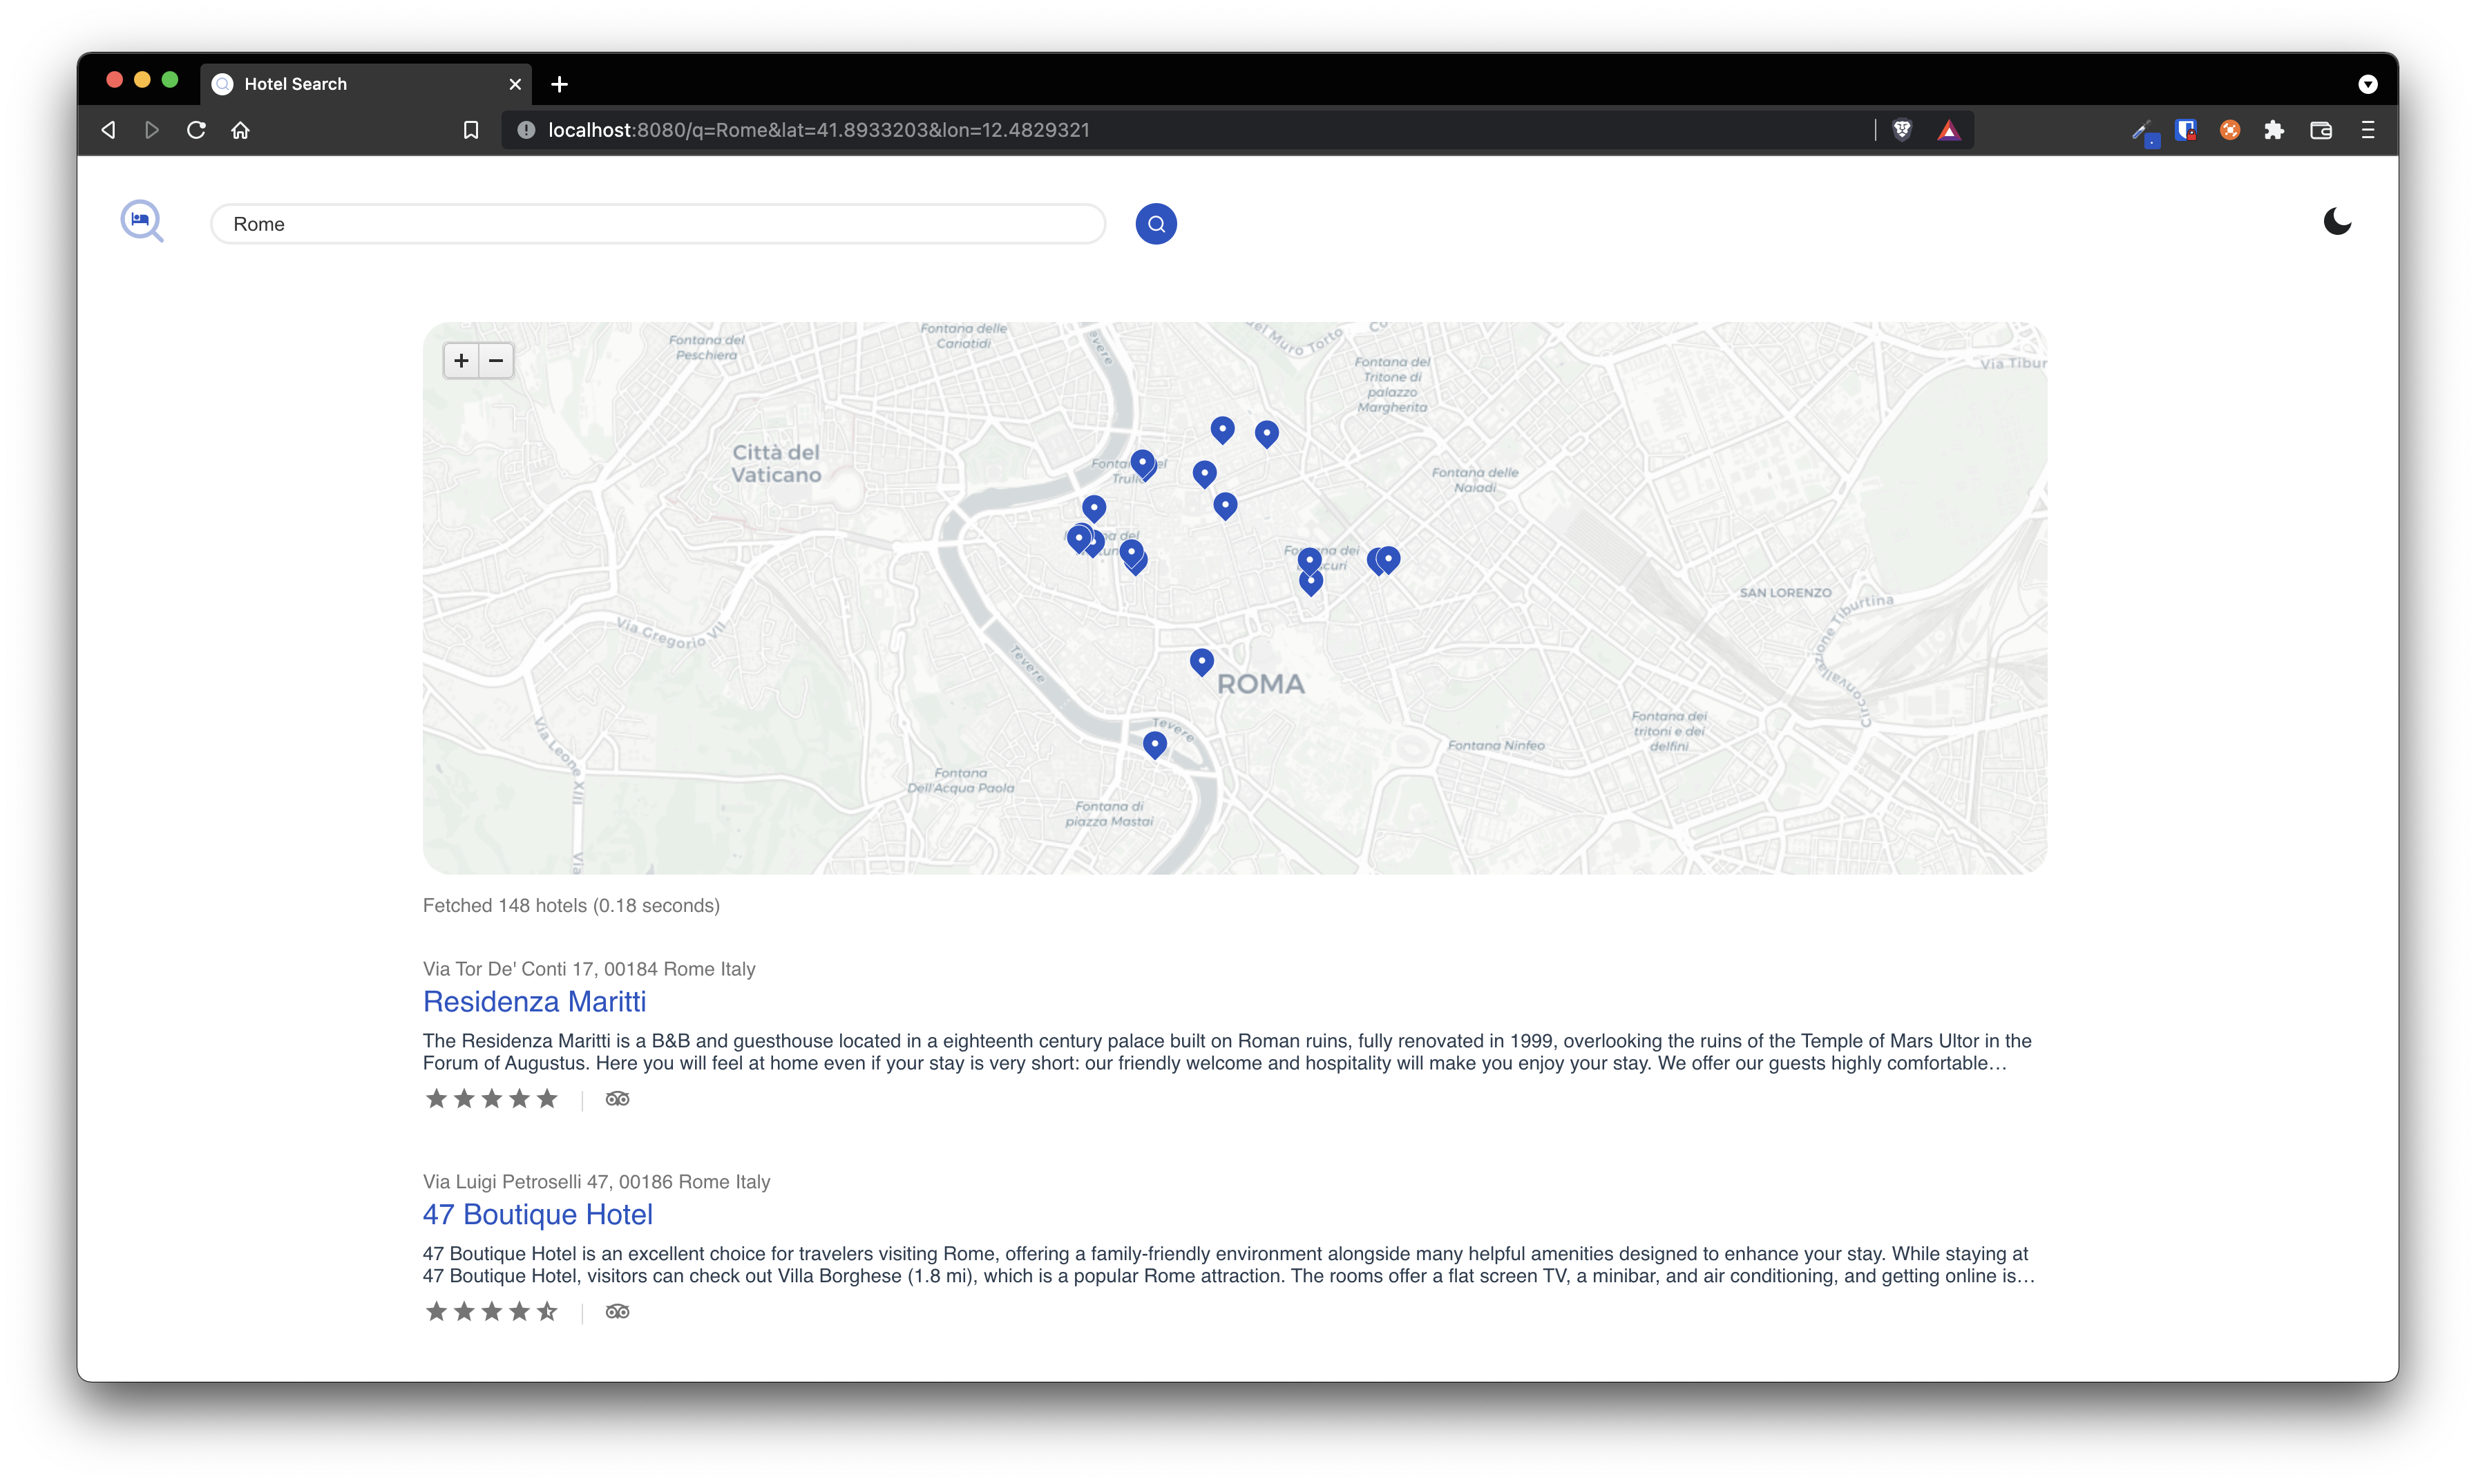
\includegraphics[width=12cm]{./results.png}
\end{center}

\subsection{Not Found Page}
This page is used in order to tell the user that the query he/she has written does not correspond to any available document. Furthermore, some suggestions are proposed to the user in order to modify the query. Such suggestions can be seen in the screen-shot below.

\begin{center}
	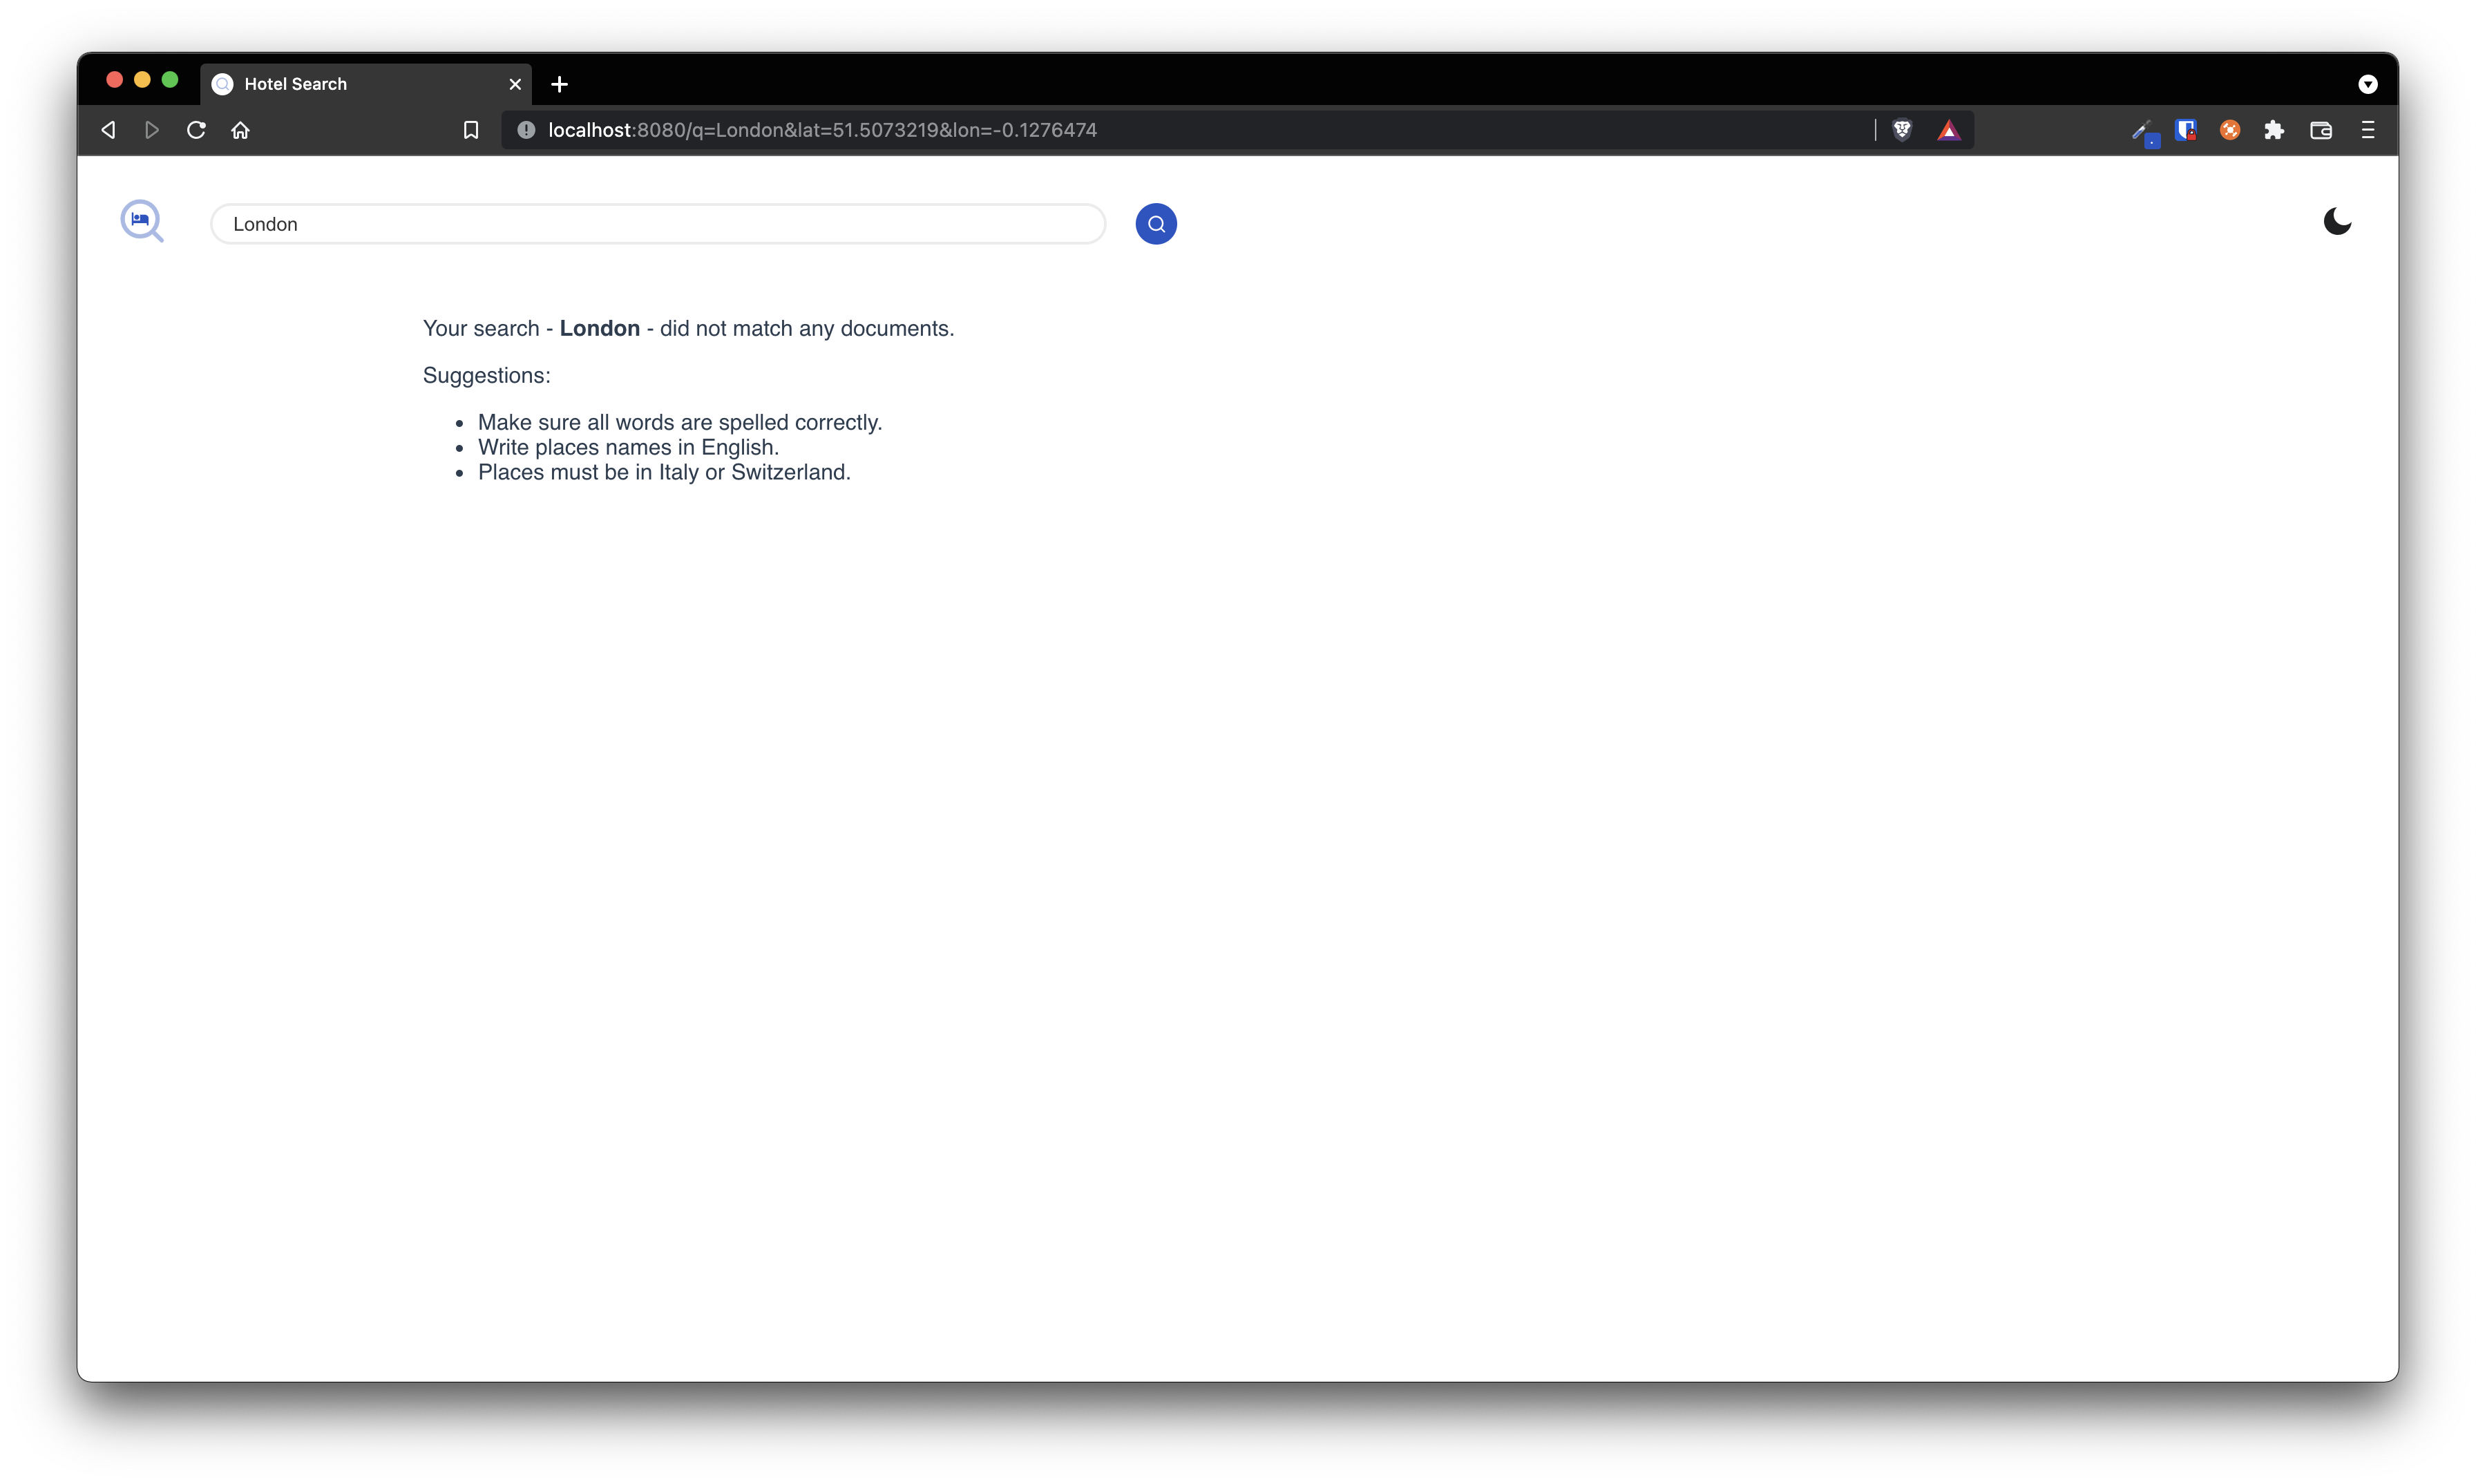
\includegraphics[width=12cm]{./not-found.png}
\end{center}

\subsection{Ad Blockers}
Something that I've noticed while working on this project, was that \textit{Ad Blockers} didn't allow the map to be visible. Thus I recommend to disable all \textit{Ad Blockers} in order to make everything work smoothly.

\section{User Evaluation}
The third and final part of the project was to perform a user evaluation of our system. In order to do so, I've chosen five tasks and gave them to three test users. These tasks were chosen because they cover all of the features of the search engine. The following were the performed tasks:

\begin{itemize}
	\item Find the three most relevant hotels when looking for "Rome".
	\item Hover on a marker located on the map. Is that hotel present in the top twenty results -- i.e. in the first page?
	\item Visit the fourth result page of the hotels.
	\item Change the query from "Rome" to "Milan". Are the results still relevant to the query?
	\item Search for a place that is outside of both Italy and Switzerland. Is the displayed page relevant to the query?
\end{itemize}
The users, after completing the above tasks, were given a series of parameters to evaluate. These parameters were: \textit{usability}, \textit{relevance} and \textit{interface}. Each evaluation is in a scale of one to five, where one means that the search engine is respectively: not usable, the results are not relevant to the query, and the interface is not up to par. On the other hand, five means that the search engine is respectively: usable, results are relevant, and the interface is well done.

\subsection{User One}
The fist user, after completing the five tasks, gave the following evaluation of the system:

\begin{table}[H]
	\centering
	\begin{tabular}{|c|c|c|} \hline 
		\textbf{Usability} & \textbf{Relevance} & \textbf{Interface}  \\ \hline
		4.5 & 5 & 5 \\
		\hline
	\end{tabular}
\end{table}

\subsection{User Two}
The second user, after completing the five tasks, gave the following evaluation of the system:

\begin{table}[H]
	\centering
	\begin{tabular}{|c|c|c|} \hline 
		\textbf{Usability} & \textbf{Relevance} & \textbf{Interface}  \\ \hline
		4 & 5 & 5 \\
		\hline
	\end{tabular}
\end{table}

\subsection{User Three}
The third and final user user, after completing the five tasks, gave the following evaluation of the system:

\begin{table}[H]
	\centering
	\begin{tabular}{|c|c|c|} \hline 
		\textbf{Usability} & \textbf{Relevance} & \textbf{Interface}  \\ \hline
		5 & 4.75 & 5 \\
		\hline
	\end{tabular}
\end{table}

\end{document}























